\documentclass[14pt]{extbook}
\usepackage{multicol, enumerate, enumitem, hyperref, color, soul, setspace, parskip, fancyhdr} %General Packages
\usepackage{amssymb, amsthm, amsmath, bbm, latexsym, units, mathtools} %Math Packages
\everymath{\displaystyle} %All math in Display Style
% Packages with additional options
\usepackage[headsep=0.5cm,headheight=12pt, left=1 in,right= 1 in,top= 1 in,bottom= 1 in]{geometry}
\usepackage[usenames,dvipsnames]{xcolor}
\usepackage{dashrule}  % Package to use the command below to create lines between items
\newcommand{\litem}[1]{\item#1\hspace*{-1cm}\rule{\textwidth}{0.4pt}}
\pagestyle{fancy}
\lhead{Progress Quiz 4}
\chead{}
\rhead{Version A}
\lfoot{6286-1986}
\cfoot{}
\rfoot{Fall 2020}
\begin{document}

\begin{enumerate}
\litem{
Solve the radical equation below. Then, choose the interval(s) that the solution(s) belongs to.\[ \sqrt{28 x^2 + 14} - \sqrt{-42 x} = 0 \]\begin{enumerate}[label=\Alph*.]
\item \( x \in [-0.55,-0.14] \)
\item \( x \in [-1.08,-0.59] \)
\item \( x_1 \in [-1.08, -0.59] \text{ and } x_2 \in [-1.8,0.1] \)
\item \( \text{All solutions lead to invalid or complex values in the equation.} \)
\item \( x_1 \in [0.45, 0.56] \text{ and } x_2 \in [0,2.2] \)

\end{enumerate} }
\litem{
Choose the equation of the function graphed below.
\begin{center}
    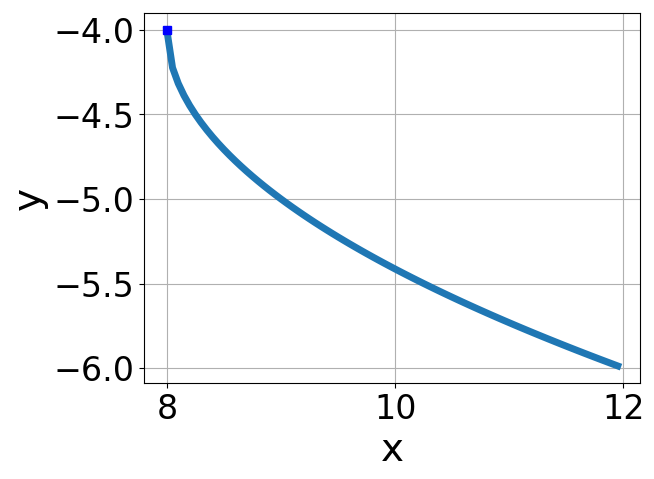
\includegraphics[width=0.5\textwidth]{../Figures/radicalGraphToEquationA.png}
\end{center}
\begin{enumerate}[label=\Alph*.]
\item \( f(x) = \sqrt[3]{x + 8} + 4 \)
\item \( f(x) = - \sqrt[3]{x - 8} + 4 \)
\item \( f(x) = - \sqrt[3]{x + 8} + 4 \)
\item \( f(x) = \sqrt[3]{x - 8} + 4 \)
\item \( \text{None of the above} \)

\end{enumerate} }
\litem{
Solve the radical equation below. Then, choose the interval(s) that the solution(s) belongs to.\[ \sqrt{35 x^2 + 21} - \sqrt{64 x} = 0 \]\begin{enumerate}[label=\Alph*.]
\item \( x \in [0.8,4.1] \)
\item \( x_1 \in [-0.6, 0.9] \text{ and } x_2 \in [0.4,4.4] \)
\item \( x_1 \in [-1.5, -0.2] \text{ and } x_2 \in [-4.43,0.57] \)
\item \( x \in [-0.6,0.9] \)
\item \( \text{All solutions lead to invalid or complex values in the equation.} \)

\end{enumerate} }
\litem{
Solve the radical equation below. Then, choose the interval(s) that the solution(s) belongs to.\[ \sqrt{9 x + 9} - \sqrt{5 x - 3} = 0 \]\begin{enumerate}[label=\Alph*.]
\item \( x \in [-1.6,-1.16] \)
\item \( x_1 \in [-4.22, -2.68] \text{ and } x_2 \in [-2,0] \)
\item \( x_1 \in [-1.44, -0.97] \text{ and } x_2 \in [-0.4,6.6] \)
\item \( \text{All solutions lead to invalid or complex values in the equation.} \)
\item \( x \in [-4.22,-2.68] \)

\end{enumerate} }
\litem{
What is the domain of the function below?\[ f(x) = \sqrt[3]{-7 x - 4} \]\begin{enumerate}[label=\Alph*.]
\item \( (-\infty, \infty) \)
\item \( \text{The domain is } (-\infty, a], \text{   where } a \in [-4, -1.4] \)
\item \( \text{The domain is } [a, \infty), \text{   where } a \in [-5, -1.3] \)
\item \( \text{The domain is } (-\infty, a], \text{   where } a \in [-1, 2.8] \)
\item \( \text{The domain is } [a, \infty), \text{   where } a \in [-1.3, 2.1] \)

\end{enumerate} }
\litem{
What is the domain of the function below?\[ f(x) = \sqrt[3]{5 x - 7} \]\begin{enumerate}[label=\Alph*.]
\item \( \text{The domain is } (-\infty, a], \text{   where } a \in [0.6, 1.1] \)
\item \( (-\infty, \infty) \)
\item \( \text{The domain is } (-\infty, a], \text{   where } a \in [0.9, 3.6] \)
\item \( \text{The domain is } [a, \infty), \text{   where } a \in [0.05, 0.91] \)
\item \( \text{The domain is } [a, \infty), \text{   where } a \in [1.04, 1.72] \)

\end{enumerate} }
\litem{
Choose the graph of the equation below.\[ f(x) = - \sqrt[3]{x - 10} - 6 \]\begin{enumerate}[label=\Alph*.]
\begin{multicols}{2}\item 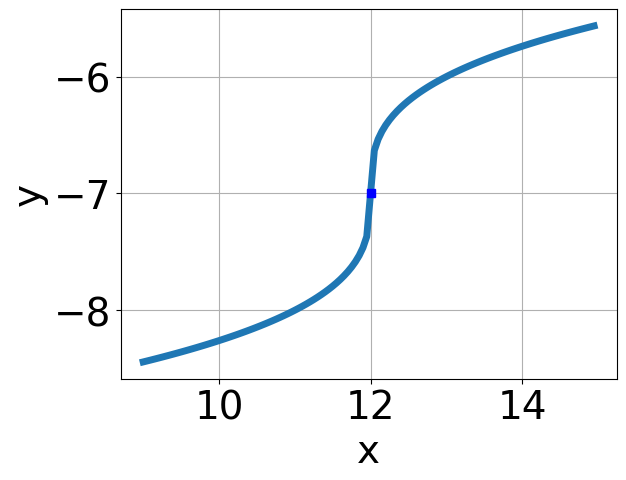
\includegraphics[width = 0.3\textwidth]{../Figures/radicalEquationToGraphAA.png}\item 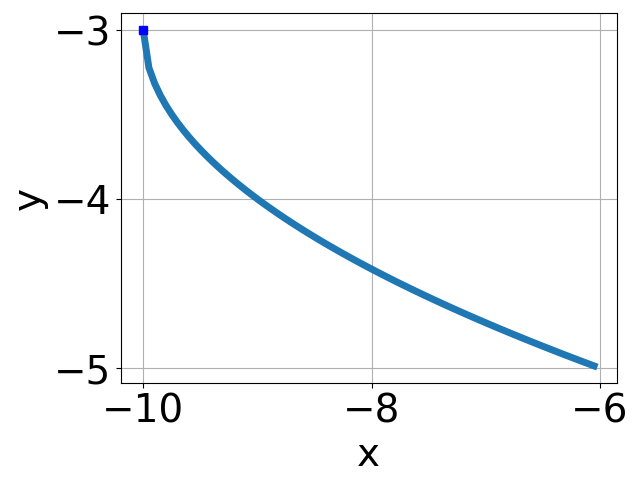
\includegraphics[width = 0.3\textwidth]{../Figures/radicalEquationToGraphBA.png}\item 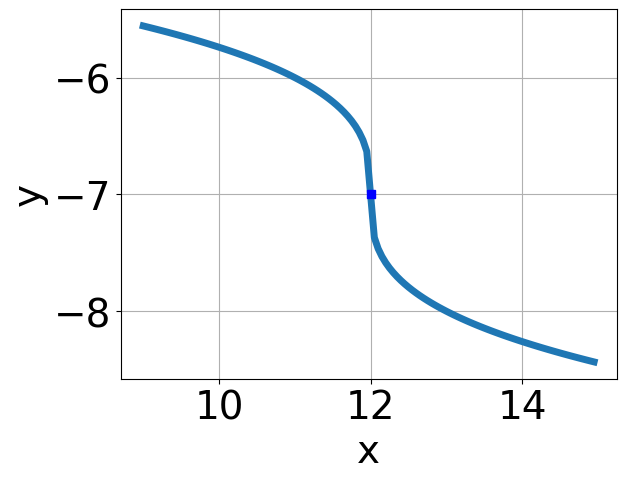
\includegraphics[width = 0.3\textwidth]{../Figures/radicalEquationToGraphCA.png}\item 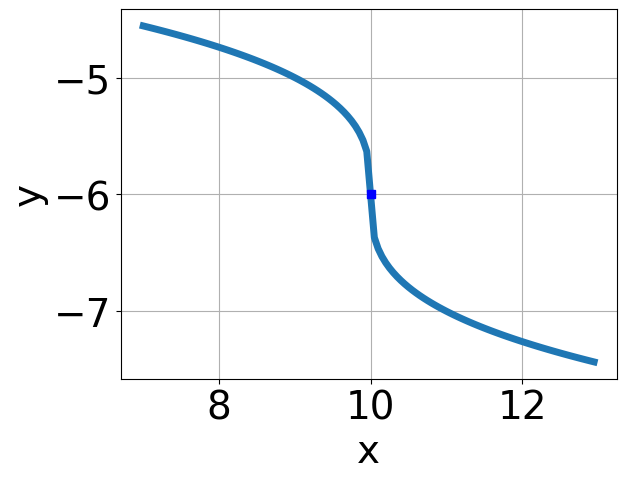
\includegraphics[width = 0.3\textwidth]{../Figures/radicalEquationToGraphDA.png}\end{multicols}\item None of the above.
\end{enumerate} }
\litem{
Solve the radical equation below. Then, choose the interval(s) that the solution(s) belongs to.\[ \sqrt{-2 x - 5} - \sqrt{3 x + 6} = 0 \]\begin{enumerate}[label=\Alph*.]
\item \( x_1 \in [-2.8, -2.21] \text{ and } x_2 \in [-2.18,-1.85] \)
\item \( x \in [-0.13,0.29] \)
\item \( x_1 \in [-2.8, -2.21] \text{ and } x_2 \in [-2.38,-2.1] \)
\item \( x \in [-2.39,-2.07] \)
\item \( \text{All solutions lead to invalid or complex values in the equation.} \)

\end{enumerate} }
\litem{
Choose the graph of the equation below.\[ f(x) = \sqrt{x - 12} - 4 \]\begin{enumerate}[label=\Alph*.]
\begin{multicols}{2}\item 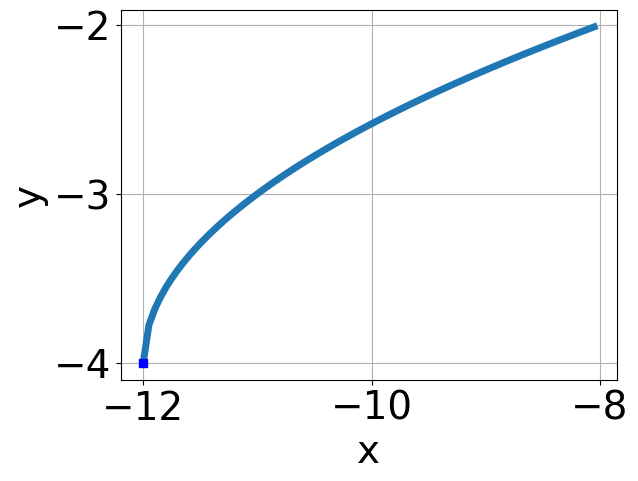
\includegraphics[width = 0.3\textwidth]{../Figures/radicalEquationToGraphCopyAA.png}\item 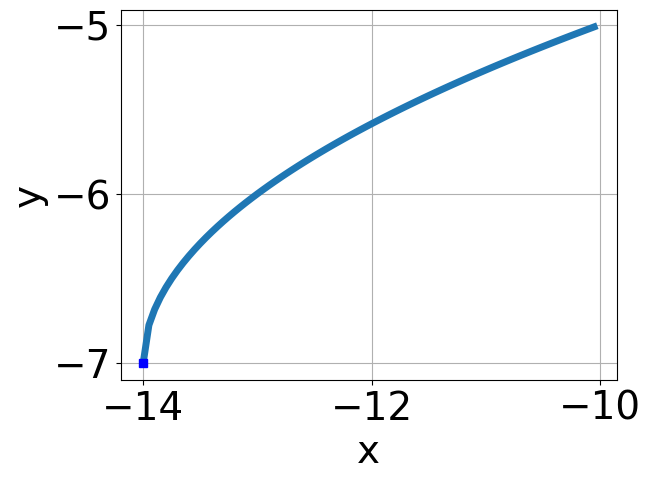
\includegraphics[width = 0.3\textwidth]{../Figures/radicalEquationToGraphCopyBA.png}\item 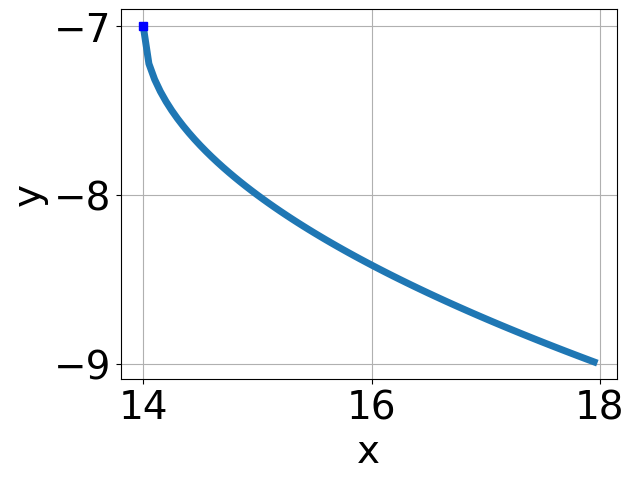
\includegraphics[width = 0.3\textwidth]{../Figures/radicalEquationToGraphCopyCA.png}\item 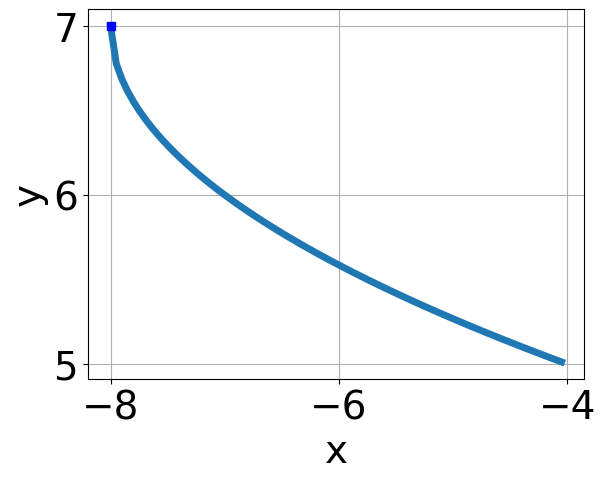
\includegraphics[width = 0.3\textwidth]{../Figures/radicalEquationToGraphCopyDA.png}\end{multicols}\item None of the above.
\end{enumerate} }
\litem{
Choose the equation of the function graphed below.
\begin{center}
    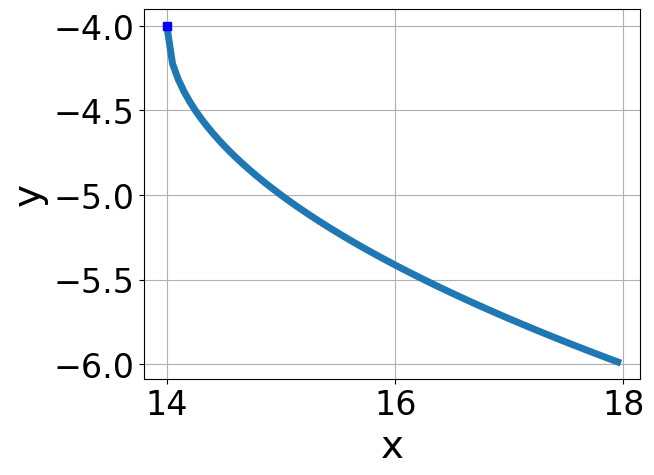
\includegraphics[width=0.5\textwidth]{../Figures/radicalGraphToEquationCopyA.png}
\end{center}
\begin{enumerate}[label=\Alph*.]
\item \( f(x) = - \sqrt{x + 12} - 7 \)
\item \( f(x) = \sqrt{x + 12} - 7 \)
\item \( f(x) = \sqrt{x - 12} - 7 \)
\item \( f(x) = - \sqrt{x - 12} - 7 \)
\item \( \text{None of the above} \)

\end{enumerate} }
\end{enumerate}

\end{document}